\documentclass[12pt,a4paper]{article}

% ─── Page Layout ───────────────────────────────────────────────────────────────
\usepackage[a4paper, margin=0.8in, headheight=14pt]{geometry}

% ─── Fonts (XeLaTeX) ───────────────────────────────────────────────────────────
\usepackage{fontspec}
\usepackage{unicode-math}
\setmainfont{TeX Gyre Pagella}
\setmonofont[Scale=0.88]{TeX Gyre Cursor}
\setmathfont{Latin Modern Math}

% ─── Packages ──────────────────────────────────────────────────────────────────
\usepackage{xcolor}
\usepackage{colortbl}
\usepackage{titlesec}
\usepackage{enumitem}
\usepackage{tabularx}
\usepackage{booktabs}
\usepackage{array}
\usepackage{amsmath}
\usepackage{tikz}
\usetikzlibrary{shapes.geometric, arrows.meta, positioning, calc, fit, decorations.pathreplacing, decorations.pathmorphing}
\usepackage{tcolorbox}
\tcbuselibrary{skins, breakable}
\usepackage{hyperref}
\usepackage{fancyhdr}
\usepackage{graphicx}
\usepackage{microtype}
\hyphenpenalty=10000
\exhyphenpenalty=10000
\sloppy
\usepackage{caption}
\usepackage{setspace}
\usepackage{multirow}
\usepackage{tocloft}

% ─── Q&A helper ────────────────────────────────────────────────────────────────
\newcommand{\Q}[1]{\textbf{#1}\par\noindent\ignorespaces}

% ─── Colour Palette ────────────────────────────────────────────────────────────
\definecolor{myred}{RGB}{196,30,58}
\definecolor{mydark}{RGB}{30,30,50}
\definecolor{mygreen}{RGB}{14,120,80}
\definecolor{myteal}{RGB}{0,130,140}
\definecolor{myamber}{RGB}{180,100,0}
\definecolor{mypurple}{RGB}{100,30,160}
\definecolor{mygray}{RGB}{246,247,249}
\definecolor{mgframe}{RGB}{180,185,200}
\definecolor{watermark}{RGB}{145,150,170}
\definecolor{hdrred}{RGB}{250,232,235}
\definecolor{hdrgreen}{RGB}{220,244,233}
\definecolor{hdrteal}{RGB}{220,242,244}
\definecolor{hdramber}{RGB}{253,242,215}
\definecolor{hdrpurple}{RGB}{238,228,255}
\definecolor{hdrgray}{RGB}{238,240,245}
\definecolor{rowalt}{RGB}{250,251,253}

% ─── Section Formatting ────────────────────────────────────────────────────────
\titleformat{\section}
  {\large\bfseries\color{myred}}{\thesection.}{0.5em}{}
  [\vspace{1pt}{\color{myred}\rule{\linewidth}{0.8pt}}]
\titleformat{\subsection}
  {\normalsize\bfseries\color{myteal}}{\thesubsection}{0.5em}{}
\titlespacing*{\section}{0pt}{18pt}{7pt}
\titlespacing*{\subsection}{0pt}{11pt}{4pt}

% ─── Paragraph ─────────────────────────────────────────────────────────────────
\setlength{\parindent}{0pt}
\setlength{\parskip}{4pt}

% ─── TOC Styling ───────────────────────────────────────────────────────────────
\renewcommand{\cfttoctitlefont}{\large\bfseries\color{myred}}
\renewcommand{\cftaftertoctitle}{\par\noindent{\color{myred}\rule{\linewidth}{0.8pt}}}
\setlength{\cftbeforetoctitleskip}{0pt}
\setlength{\cftaftertoctitleskip}{6pt}
\renewcommand{\cftsecfont}{\normalsize\bfseries\color{mydark}}
\renewcommand{\cftsecpagefont}{\normalsize\bfseries\color{mydark}}
\renewcommand{\cftsecleader}{\cftdotfill{\cftdotsep}}
\setlength{\cftbeforesecskip}{7pt}
\renewcommand{\cftsubsecfont}{\small\color{mydark}}
\renewcommand{\cftsubsecpagefont}{\small\color{mydark}}
\setlength{\cftbeforesubsecskip}{3pt}
\setlength{\cftsubsecindent}{1.4em}

% ─── Table helpers ─────────────────────────────────────────────────────────────
\renewcommand{\arraystretch}{1.45}
\setlength{\tabcolsep}{6pt}
\arrayrulecolor{mydark}
\newcolumntype{B}[1]{>{\small\bfseries\raggedright\arraybackslash}m{#1}}
\newcolumntype{C}[1]{>{\centering\arraybackslash}m{#1}}
\newcolumntype{Y}{>{\small\raggedright\arraybackslash}X}
\renewcommand{\tabularxcolumn}[1]{m{#1}}

% ─── Header / Footer ───────────────────────────────────────────────────────────
\pagestyle{fancy}
\fancyhf{}
\fancyhead[L]{\small\color{myred}\textbf{OE-EC704A}\;\color{mydark}--- Web Technology}
\fancyhead[R]{\small\color{myteal}\textbf{Module 8 Notes}}
\fancyfoot[C]{\small\color{mydark}\thepage}
\fancyfoot[R]{\small\color{watermark}\textit{\copyright\ Biraj}}
\renewcommand{\headrulewidth}{0.5pt}
\renewcommand{\footrulewidth}{0.3pt}

% ─── Hyperref ──────────────────────────────────────────────────────────────────
\hypersetup{
  colorlinks=true, linkcolor=myteal, urlcolor=myteal,
  pdfauthor={Biraj Sarkar},
  pdftitle={OE-EC704A --- Module 8 Notes}
}

% ─── tcolorbox styles ──────────────────────────────────────────────────────────
\tcbset{
  tikzbox/.style={
    colback=mygray, colframe=mgframe, boxrule=0.6pt, arc=4pt,
    left=8pt, right=8pt, top=6pt, bottom=6pt,
    colbacktitle=mgframe, coltitle=mydark,
    fonttitle=\small\bfseries
  },
  defbox/.style={
    colback=hdrgreen, colframe=mygreen, boxrule=0.8pt, arc=4pt,
    left=9pt, right=9pt, top=6pt, bottom=6pt,
    colbacktitle=mygreen, coltitle=white,
    fonttitle=\small\bfseries
  },
  formulabox/.style={
    colback=hdrteal, colframe=myteal, boxrule=0.8pt, arc=4pt,
    left=9pt, right=9pt, top=7pt, bottom=7pt,
    colbacktitle=myteal, coltitle=white,
    fonttitle=\small\bfseries
  },
  examplebox/.style={
    colback=hdramber, colframe=myamber, boxrule=0.8pt, arc=4pt,
    left=9pt, right=9pt, top=6pt, bottom=6pt,
    colbacktitle=myamber, coltitle=white,
    fonttitle=\small\bfseries
  },
  masonbox/.style={
    colback=hdrpurple, colframe=mypurple, boxrule=0.8pt, arc=4pt,
    left=9pt, right=9pt, top=6pt, bottom=6pt,
    colbacktitle=mypurple, coltitle=white,
    fonttitle=\small\bfseries
  },
  exambox/.style={
    colback=hdrpurple, colframe=mypurple, boxrule=1pt, arc=5pt,
    left=10pt, right=10pt, top=8pt, bottom=8pt,
    colbacktitle=mypurple, coltitle=white,
    fonttitle=\bfseries,
    breakable, title after break={\textbf{Frequently Asked / Viva Questions (contd.)}}}
}
\tcbset{breakable}

% ─── TikZ styles ───────────────────────────────────────────────────────────────
\tikzset{
  block/.style={rectangle, draw=myteal, fill=hdrteal,
    text width=2.5cm, align=center, minimum height=1.0cm,
    font=\small, rounded corners=3pt, line width=0.7pt},
  redblock/.style={rectangle, draw=myred, fill=hdrred,
    text width=2.5cm, align=center, minimum height=1.0cm,
    font=\small, rounded corners=3pt, line width=0.7pt},
  netnode/.style={rectangle, draw=myteal, fill=hdrteal,
    text width=1.8cm, align=center, minimum height=0.8cm,
    font=\small, rounded corners=3pt, line width=0.7pt},
  sumjunc/.style={circle, draw=myamber, fill=hdramber,
    minimum size=0.6cm, font=\small, line width=0.8pt},
  snode/.style={circle, draw=mypurple, fill=hdrpurple,
    minimum size=0.55cm, font=\footnotesize, line width=0.7pt},
  arrow/.style={-Stealth, thick, color=mydark},
  redarrow/.style={-Stealth, thick, color=myred},
  line/.style={thick, color=mydark}
}

% ═══════════════════════════════════════════════════════════════════════════════
\begin{document}
% ═══════════════════════════════════════════════════════════════════════════════

\begin{center}
  {\LARGE\bfseries\color{myred} OE-EC704A --- Web Technology}\\[5pt]
  {\normalsize\color{mydark} Semester VII \quad$\bullet$\quad 3L:0T:0P \quad$\bullet$\quad 3 Credits}\\[3pt]
  {\normalsize\color{myteal}\textbf{Module 8 Exam Notes: Java Utility Package (Collections Framework)}}\\[3pt]
  {\small\color{mydark} CGEC \;$|$\; B.Tech ECE (2023--27) \;$|$\; \textit{Biraj Sarkar}}
\end{center}
\noindent{\color{myred}\rule{\linewidth}{1.5pt}}
\vspace{2pt}

\hypersetup{linkcolor=mydark}
\tableofcontents
\hypersetup{linkcolor=myteal}
\newpage

% ===============================================================================
\section{Java Collections Framework Overview}
% ===============================================================================

The Collections Framework, declared inside the \texttt{java.util} package, provides a unified architecture to store and manipulate a group of objects.

\begin{tcolorbox}[defbox, title={\textbf{Core Design Benefits}}]
\begin{itemize}[leftmargin=*, itemsep=3pt]
  \item Reduces programming effort by providing standard data structures.
  \item Boosts speed and quality via high-performance, optimized implementations.
  \item Promotes software reuse by offering polymorphic operations.
\end{itemize}
\end{tcolorbox}

\subsection{Core Interfaces}
The framework is structured hierarchically around a set of core interfaces:
\begin{itemize}[leftmargin=*, itemsep=4pt]
  \item \textbf{\texttt{Collection}:} The root interface defining basic operations (size, add, remove, clear).
  \item \textbf{\texttt{List}:} Extends \texttt{Collection}. Represents an ordered sequence of elements that can contain duplicates. Supports index-based access.
  \item \textbf{\texttt{Set}:} Extends \texttt{Collection}. A collection that cannot contain duplicate elements, modeling mathematical sets.
  \item \textbf{\texttt{Queue}:} Extends \texttt{Collection}. Designed to hold elements prior to processing (typically FIFO).
\end{itemize}

% ===============================================================================
\section{ArrayList vs. LinkedList}
% ===============================================================================

\par\noindent
{\renewcommand{\arraystretch}{1.5}%
\begin{tabularx}{\linewidth}{|B{3.2cm}|Y|Y|}
\hline
\textbf{Metric} & \textbf{\texttt{ArrayList}} & \textbf{\texttt{LinkedList}} \\
\hline
\textbf{Internal Structure} & Dynamically resizing array. & Doubly linked list nodes. \\
\hline
\textbf{Access Time} & $O(1)$ random access (index-based). & $O(n)$ search access (sequential traverse). \\
\hline
\textbf{Insertion/Deletion} & $O(n)$ (requires element shifts). & $O(1)$ if pointer is located. \\
\hline
\textbf{Memory Overhead} & Low (only stores elements). & Higher (stores element and prev/next links). \\
\hline
\end{tabularx}}

\begin{tcolorbox}[tikzbox, title={ArrayList vs. LinkedList Memory Layout}]
\centering
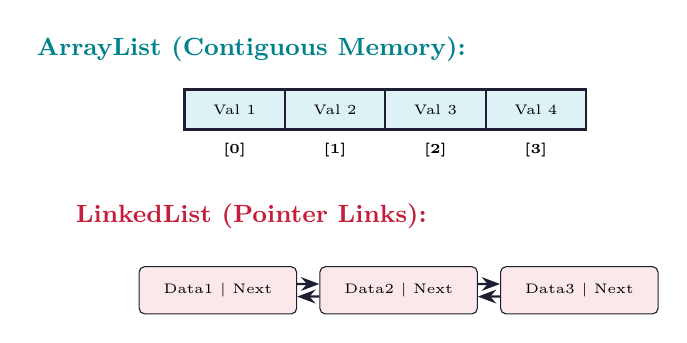
\begin{tikzpicture}[scale=0.85]
  % ArrayList
  \node[font=\small\bfseries, color=myteal] at (1,2) {ArrayList (Contiguous Memory):};
  \draw[draw=mydark, fill=hdrteal, line width=1pt] (0,0.8) rectangle (6,1.4);
  \foreach \x in {1.5, 3.0, 4.5} {
    \draw[line] (\x, 0.8) -- (\x, 1.4);
  }
  \node[font=\tiny] at (0.75, 1.1) {Val 1};
  \node[font=\tiny] at (2.25, 1.1) {Val 2};
  \node[font=\tiny] at (3.75, 1.1) {Val 3};
  \node[font=\tiny] at (5.25, 1.1) {Val 4};

  \node[font=\tiny\bfseries] at (0.75, 0.5) {[0]};
  \node[font=\tiny\bfseries] at (2.25, 0.5) {[1]};
  \node[font=\tiny\bfseries] at (3.75, 0.5) {[2]};
  \node[font=\tiny\bfseries] at (5.25, 0.5) {[3]};

  % LinkedList
  \node[font=\small\bfseries, color=myred] at (1,-0.5) {LinkedList (Pointer Links):};
  
  \node[draw=mydark, fill=hdrred, minimum width=2.0cm, minimum height=0.6cm, rounded corners=2pt] (n1) at (0.5,-1.6) {\tiny Data1 | Next};
  \node[draw=mydark, fill=hdrred, minimum width=2.0cm, minimum height=0.6cm, rounded corners=2pt] (n2) at (3.2,-1.6) {\tiny Data2 | Next};
  \node[draw=mydark, fill=hdrred, minimum width=2.0cm, minimum height=0.6cm, rounded corners=2pt] (n3) at (5.9,-1.6) {\tiny Data3 | Next};

  \draw[arrow, transform canvas={yshift=0.08cm}] (n1) -- (n2);
  \draw[arrow, transform canvas={yshift=-0.08cm}] (n2) -- (n1);
  \draw[arrow, transform canvas={yshift=0.08cm}] (n2) -- (n3);
  \draw[arrow, transform canvas={yshift=-0.08cm}] (n3) -- (n2);
\end{tikzpicture}
\tcbset{after={\color{black}}}
\end{tcolorbox}

% ===============================================================================
\section{Accessing and Iterating Collections}
% ===============================================================================

Java provides two primary mechanisms to traverse through collection elements:

\subsection{The Iterator Interface}
An iterator provides sequential access to collection elements. It is retrieved using \texttt{iterator()} method on any Collection object.
\begin{verbatim}
ArrayList<String> list = new ArrayList<>();
list.add("Java");
list.add("HTML");

Iterator<String> itr = list.iterator();
while (itr.hasNext()) {
    String element = itr.next();
    System.out.println(element);
}
\end{verbatim}
\begin{itemize}[leftmargin=*, itemsep=3.5pt]
  \item \textbf{Methods:} \texttt{hasNext()} (returns true if more elements exist), \texttt{next()} (returns next element), and \texttt{remove()} (removes current element safely during iteration).
  \item \textbf{Fail-Fast Behavior:} Iterators on standard collections like ArrayList throw a \texttt{ConcurrentModificationException} if the collection is structurally modified (add/remove) outside the iterator's own methods during iteration.
\end{itemize}

\subsection{The For-Each Statement}
Introduced in Java 5, the enhanced \texttt{for} loop (for-each) provides a cleaner syntax to iterate over arrays and collections:
\begin{verbatim}
for (String element : list) {
    System.out.println(element);
}
\end{verbatim}
Internally, the compiler translates this syntax into standard Iterator-based code for objects implementing the \texttt{java.lang.Iterable} interface.

\newpage
% ===============================================================================
\begin{center}
  {\large\bfseries\color{myred} Quick Revision --- Module 8}\\[3pt]
  {\small\color{mydark} Java Utility package - Collections $|$ OE-EC704A}
\end{center}
\noindent{\color{myred}\rule{\linewidth}{1.2pt}}
\vspace{4pt}

\begin{tcolorbox}[formulabox, title={\textbf{Collection Syntax}}]
{\renewcommand{\arraystretch}{1.3}%
\begin{tabularx}{\linewidth}{l Y}
\textbf{Construct} & \textbf{Syntax and Example Usage} \\
\hline
ArrayList Declaration & \texttt{ArrayList<String> list = new ArrayList<String>();} \\
ArrayList Insert & \texttt{list.add("Java"); list.add(1, "CSS"); // inserts at index 1} \\
LinkedList Declaration & \texttt{LinkedList<Integer> lList = new LinkedList<>();} \\
Iterator Traversal & \texttt{Iterator<String> itr = list.iterator(); while(itr.hasNext()) \{ ... \}} \\
For-Each Loop & \texttt{for (String str : list) \{ System.out.println(str); \}} \\
\end{tabularx}}
\end{tcolorbox}

\begin{tcolorbox}[defbox, title={\textbf{One-Line Definitions}}]
\begin{itemize}[leftmargin=*, itemsep=2pt]
  \item \textbf{Collections Framework:} Architecture of interfaces and classes for grouping multiple objects.
  \item \textbf{ArrayList:} Resizable-array implementation of the List interface, backing elements contiguously.
  \item \textbf{LinkedList:} Doubly-linked node implementation of the List and Deque interfaces.
  \item \textbf{Iterator:} Object traversal cursor enabling forward traversal and safe element removals.
  \item \textbf{Fail-Fast Iterator:} Iterator throwing exception immediately if collection structure changes during loop.
  \item \textbf{Iterable:} Interface indicating target object can be traversed using enhanced for-each.
  \item \textbf{Generics:} Compiler feature ensuring type-safety in collections (e.g., \texttt{ArrayList<String>}).
  \item \textbf{Auto-boxing:} Implicit compiler conversion between primitives and their wrapper classes.
\end{itemize}
\tcbset{after={\color{black}}}
\end{tcolorbox}

\begin{tcolorbox}[exambox, title={\textbf{Frequently Asked / Viva Questions}}]
\begin{enumerate}[leftmargin=*, label=\textbf{Q\arabic*.}, itemsep=5pt]
  \item \Q{What is the difference between \texttt{ArrayList} and \texttt{Vector}?}
        \texttt{ArrayList} is non-synchronized, fast, and not thread-safe. \texttt{Vector} is synchronized, has thread-safe methods, and carries significant execution overhead.
        
  \item \Q{Why does a \texttt{LinkedList} consume more memory than an \texttt{ArrayList}?}
        An \texttt{ArrayList} stores elements contiguously inside a backing array. A \texttt{LinkedList} wraps each element inside a node object that also holds reference addresses for the previous and next nodes.
        
  \item \Q{What is fail-fast behavior in collections?}
        It is a JVM runtime validation that throws a \texttt{ConcurrentModificationException} if a collection is modified structurally (elements added or deleted) while an active iterator is traversing it.
        
  \item \Q{How does ArrayList grow its internal array capacity?}
        When an element is added and the array is full, ArrayList allocates a new array and copies elements. Starting from Java 10, it increases capacity by roughly $50\%$ ($\text{New Capacity} = \text{Old Capacity} + (\text{Old Capacity} \gg 1)$).
        
  \item \Q{What is the purpose of the \texttt{Iterable} interface?}
        It is the superinterface of the \texttt{Collection} interface. Implementing \texttt{Iterable} requires the class to return an \texttt{Iterator}, allowing instances to be used in the enhanced for-each loop.
        
  \item \Q{Can we store primitive data types (like \texttt{int}, \texttt{char}) inside collections?}
        No, collections only store object references. However, Java handles this automatically using \textbf{Autoboxing}, which converts primitives to their wrapper objects (e.g., \texttt{int} to \texttt{Integer}) when inserted.
        
  \item \Q{What is the difference between \texttt{Iterator} and \texttt{ListIterator}?}
        \texttt{Iterator} can traverse any Collection in a forward direction. \texttt{ListIterator} can only traverse Lists, but supports bidirectional traversal (forward and backward) and element modifications.
        
  \item \Q{Which List implementation is preferred for frequent search operations?}
        \texttt{ArrayList} is preferred because it supports $O(1)$ constant time lookup via index-based access, whereas \texttt{LinkedList} requires $O(n)$ linear traversal.
        
  \item \Q{Which List implementation is preferred for frequent insertions at the beginning of the list?}
        \texttt{LinkedList} is preferred. Inserting at the beginning requires only updating two node pointers ($O(1)$), whereas \texttt{ArrayList} requires shifting all existing elements, taking $O(n)$ time.
        
  \item \Q{What is the difference between \texttt{List} and \texttt{Set} interfaces?}
        A \texttt{List} maintains insertion order and can contain duplicate elements. A \texttt{Set} is unordered and cannot contain duplicate elements.
\end{enumerate}
\end{tcolorbox}

\begin{tcolorbox}[tikzbox, title={ArrayList vs. LinkedList operations complexity}]
\centering
{\renewcommand{\arraystretch}{1.45}%
\begin{tabularx}{\linewidth}{|B{3.2cm}|Y|Y|}
\hline
\textbf{Operation} & \textbf{ArrayList} & \textbf{LinkedList} \\
\hline
\textbf{Get by Index} & $O(1)$ constant time. & $O(n)$ linear traversal. \\
\hline
\textbf{Insert/Delete (Start)} & $O(n)$ shift overhead. & $O(1)$ pointer change. \\
\hline
\textbf{Insert/Delete (End)} & $O(1)$ amortized. & $O(1)$ tail reference update. \\
\hline
\textbf{Memory consumption} & Low (consecutive slots). & High (two references per node). \\
\hline
\end{tabularx}}
\tcbset{after={\color{black}}}
\\
\end{tcolorbox}

\end{document}
